\section{Auswertung}

\subsection{Überprüfung der Bragg-Bedingung}
Zur Überprüfung der Bragg-Bedingung wird der Kristall auf einen festen Winkel von  $\theta= 14\,\mathrm{°}$ gestellt. 
Dadurch beträgt der Sollwinkel des Maximums die Werte  $\theta_\text{GM,theorie}=2\theta=28\,\mathrm{°}$, um den reflextierten Strahl einzufangen.\\
Die Messwerte davon sind in Tabelle \ref{tab:Braggbedingung} aufgeführt und in Abbildung \ref{fig:Bragg} veranschaulicht.
Aus der Abbildung \ref{fig:Bragg} wird der Winkel des Maximums abgelesen. Dieser beträgt $\theta_\text{GM}=28,2\,\mathrm{°}$.
\begin{table}[H]
    \centering
    \caption{Messdaten für die Überprüfung der Bragg-Bedingung.}
    \label{tab:Braggbedingung}
    \begin{tabular}{|c| c || c |c|}
    \toprule
    $\theta_\text{GM}/\mathrm{°}$ & $N/(\mathrm{Imp/s})$ & $\theta_\text{GM}/\mathrm{°}$ & $N/(\mathrm{Imp/s})$\\
    \midrule
    26,0 & 	56,0 &28,1&215,0\\
    26,1 & 	58,0 &28,2&208,0\\
    26,2 & 	54,0 &28,3&215,0\\
    26,3 &	62,0 &28,4&208,0\\
    26,4 &	58,0 &28,5&189,0\\
    26,5 &	68,0 &28,6&189,0\\
    26,6 &	72,0 &28,7&176,0\\
    26,7 &	83,0 &28,8&164,0\\
    26,8 &	89,0 &28,9&149,0\\
    26,9 &	95,0 &29,0&138,0\\
    27,0 &	105,0&29,1 &125,0\\
    27,1 &	119,0&29,2 &111,0\\ 
    27,2 &	125,0&29,3 &107,0\\
    27,3 &	141,0&29,4 &95,0\\
    27,4 &	154,0& 29,5&77,0\\
    27,5 &	157,0&29,6&73,0\\
    27,6 &	166,0&29,7 &58,0\\
    27,7 &	180,0&29,8 &56,0\\
    27,8 &	188,0&29,9 &53,0\\
    27,9 &	211,0&30,0 &53,0\\
    28,0 &	212,0& &\\              
    \bottomrule
    \end{tabular}
\end{table}

\begin{figure}[H]
    \centering
    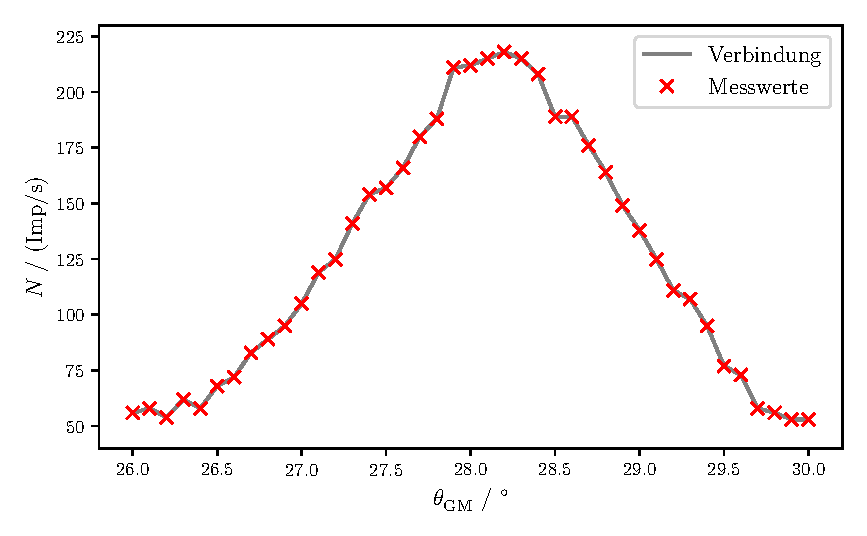
\includegraphics{Bragg.pdf}
    \caption{Überprüfung der Bragg-Bedingung.}
    \label{fig:Bragg}
  \end{figure}
  \newpage 
\subsection{Analyse eines Emissionsspektrums der Kupfer-Röntgenröhre}
Das Röntgenspektrum \cite{AL} der Kupfer Röntgenröhre wird in 0,1°-Schritten in Bereich  von \(8° \leq \theta \leq 25°\) und in Abbildung \ref{fig:EmissionCu} veranschaulicht.

\begin{figure}[H]
    \centering
    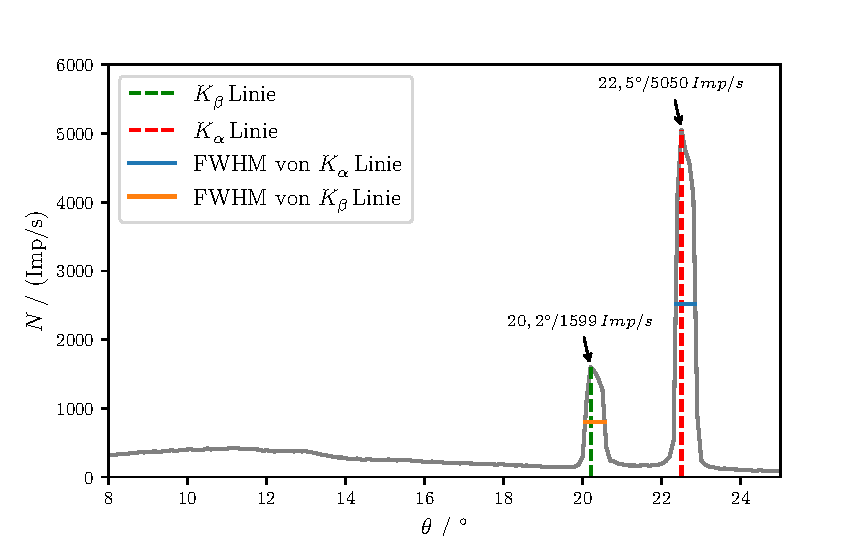
\includegraphics{EmissionCu.pdf}
    \caption{Emissionspektrum.}
    \label{fig:EmissionCu}
  \end{figure}


Aus der Abbildung \ref{fig:EmissionCu} werden Intensitäten und Kristallwinkeln bei dem ersten und zweiten Bergen (entsprechen für $K_\alpha$- und $K_\beta$-Linie von Kupfer Emissionspektrum) notiert.

Für $K_\alpha$-Linie: \(\theta=22,5°\); \(N=5050 \, \mathrm{Imp/s}\).

Für $K_\beta$-Linie: \(\theta=20,2°\); \(N=1599 \,\mathrm{Imp/s}\). \\

Die entsprechende Energien werden mit der Formel
\begin{equation}
  E = \frac{hc}{\lambda}\\
 \end{equation}
mit den durch die Formel (9) gerechneten Wellenlängen $\lambda$
bestimmt. Es ergeben sich
\begin{align*}
  E_\alpha &= 8,059\,\mathrm{keV}\\
  E_\beta &= 8,931 \,\mathrm{keV}.\\
\end{align*}
Die minimale Wellenlänge bzw. die maximale Energie des Bremsberges können nicht aus den gemesenen Daten entnommen werden. 
Der Grund dafür ist: Beim dem Teil des Versuches wird das Emissionspektrum in 0,1°-Schritten in einem Winkelbereich von \(8° \leq \theta \leq 25°\) aufgenommen.
Der Winkel, bei dem die durch die Formel (1) berechnete minimale Wellenlänge sich befindet, beträgt 5,05°. Dieser Winkel wird mit Hilfe der Formel (9) bestimmt.
Daher liegt der Winkel 5,05° au{\ss}erhalb des Winkelbereichs des Versuches.
\paragraph{}
Aus der Abbildung \ref{fig:EmissionCu} werden die Halbwertsbreite (Full Width at Half Maximum) für die Cu-$K_\alpha-$ und Cu-$K_\beta-$Linie bestimmt.
\paragraph{}
$K_\alpha$-Linie: $\text{FWHM}_\alpha= 0,494 \,\mathrm{°}$ 

\,\,\,\,\,\,\,\,\,\(\Delta E_{\text{FWHM},\alpha}=166,231\,\mathrm{eV}\) bei \(\theta_{\text{min},\alpha}=22,355°\); \(\theta_{\text{max},\alpha}=22,849°\).\\

$K_\beta$-Linie: $\text{FWHM}_\beta= 0,495 \,\mathrm{°}$

\,\,\,\,\,\,\,\,\,\(\Delta E_{\text{FWHM},\beta}=207,488\,\mathrm{eV}\) bei \(\theta_{\text{min},\beta}=20,061°\); \(\theta_{\text{max},\beta}=20,556°\). \\ 

$\Delta E$ wird mit der Formel
\begin{equation}
    \Delta E_{\text{FWHM}} = E(\lambda_{\text{min}}) -E(\lambda_{\text{max}})\\
   \end{equation}
berechnet, wobei\\ 
-die Wellenlängen ($\lambda_{\text{min}}\, \text{bei}\, \theta_{\text{min}}$, $\lambda_{\text{max}}\, \text{bei}\, \theta_{\text{max}}$) mit Formel (9) bestimmt werden:
\begin{align*}
  \lambda_{\text{min},\alpha}&=153,203\,\mathrm{pm}  & \lambda_{\text{max},\alpha}&=156,409 \,\mathrm{pm} \\
  \lambda_{\text{min},\beta}&=138,169\,\mathrm{pm}  & \lambda_{\text{max},\beta}&=141,322\,\mathrm{pm}, \\
\end{align*}
-die Energien ($E(\lambda_{\text{min}})$, $E(\lambda_{\text{max}})$) mit Formel (10) bestimmt werden:
\begin{align*}
E_{\lambda_{\text{min},\alpha}}&=8,109\,\mathrm{keV} & E_{\lambda_{\text{max},\alpha}}&=7,943\,\mathrm{keV}\\
E_{\lambda_{\text{min},\beta}}&=8,992\,\mathrm{keV} & E_{\lambda_{\text{max},\beta}}&= 8,791\,\mathrm{keV}.\\
\end{align*}
\paragraph{}
Das Auflösungsvermögen der Apparatur beider Linien werden durch die Formel
\begin{equation}
    A = \frac{E_K}{\Delta E_{\text{FWHM}}}\\
   \end{equation}
ermittelt und ergeben sich zu
\begin{align*}
    A_\alpha &= 48,481\\
    A_\beta &= 43,043.\\
  \end{align*}

Die Energiedifferenz zwischen die $K_\alpha$- und $K_\beta$-Linie beträgt 
\begin{align*}
    \Delta E = E_{K,\alpha}-E_{K,\beta} = 872\, \mathrm{eV}.
  \end{align*}

\paragraph{}
Die Abschirmkonstanten $\sigma_1$, $\sigma_2$ und $\sigma_3$ aus den Emissionsenergien der Cu-$K_\alpha-$ und Cu-$K_\beta-$Linie werden mit folgender Formel bestimmt mit $n= 1$, $m= 2$ und $l= 3$.
\begin{gather}
E_{K,\text{abs}} = R_\infty(Z-\sigma_1)^2\\
E_{K,\alpha} = R_\infty\Bigl(\frac{1}{n}\Bigr)^2 \cdot (Z-\sigma_1)^2 -R_\infty\Bigl(\frac{1}{m}\Bigr)^2 \cdot (Z-\sigma_2)^2 \\
E_{K,\beta} =  R_\infty\Bigl(\frac{1}{n}\Bigr)^2 \cdot (Z-\sigma_1)^2 -R_\infty\Bigl(\frac{1}{l}\Bigr)^2 \cdot (Z-\sigma_3)^2 
\end{gather}
dabei ist $R_\infty$ die Rydbergenergie und $Z$ die Ordnungszahl.\\

Die Abschirmkonstanten lauten 
\begin{align*}
    \sigma_{1,\text{theorie}} &=3,299 & \text{für}\, E{^\text{Lit}_{K,\text{abs}}}&=8,988\,\mathrm{keV} \intertext{%
\begin{flushright}
\cite{XT}
\end{flushright}
    }\\
    \sigma_2 &=12,480& \text{für}\, E_{K,\alpha} &= 8,059\,\mathrm{keV}\\
    \sigma_3 &=22,896& \text{für}\, E_{K,\beta} &=8,931 \,\mathrm{keV}.\\
  \end{align*}


\subsection{Anaylse der Absorptionsspektren}
\subsubsection{Das Absorptionsspektren der Absorber}
Die Messwerte zum Absorptionsspektrum von Zink, Gallium, Brom, Rubidium, Stronium, Zirkronium sind in Tabellen aufgeführt und in Abbildungen veranschaulicht. (siehe Anhang)\\
Zur Bestimmung der Abschirmkonstante $\sigma_K$ ist "Mitte der Kante" benötigt.
 Der zugehörige Winkel $\bar{\theta}$ der Absorptionsenergie $E_{K,\text{abs}}$ wird aus den Winkel $\theta{^{\text{max}} _K}$ mit dem Intensitätsmaximun $I{^{\text{max}} _K}$ und den Winkel $\theta{^{\text{min}} _K}$ mit dem Intensitätsmaximun $I{^{\text{min}} _K}$ ermittelt
\begin{equation}
    \bar{\theta_K}= \frac{\theta{^{\text{max}} _K}-\theta{^{\text{min}} _K}}{2}.\\
   \end{equation}
Die Absorptionsenergie $E_{K,\text{abs}}$ wird mit der Gleichung (10) bestimmt, wobei die entspechende Wellenlängen mit der Formel (9) gerechnet werden.\\
Die Abschirmkonstante der Absorber wird mit der Gleichung (7) gerechnet.\\
Die aus der Rechnungen erhaltenen Werte sind in Tabelle \ref{tab:Berechnetwerte} aufgeführt.
\begin{table}[H]
    \centering
    \caption{Berechnete Werte für die Absorber.}
    \label{tab:Berechnetwerte}
    \begin{tabular}{|l|c|c|c|c|c|c|}
      \toprule
        {} & $Z$  &$\theta{^{\text{max}} _K}/\mathrm{°}$   & $\theta{^{\text{min}} _K}/\mathrm{°}$   & $\bar{\theta_K}/\mathrm{°}$ & $E_{K,\text{abs}}/\mathrm{keV} $ & $\sigma_K$\\
        \midrule
        $\text{Zn}$&30&19,0&18,4&18,7&9,619&3,615\\
        $\text{Ga}$&31&17,8&17,1&14,45&10,284&3,731\\
        $\text{Br}$&35&13,5&13,0&13,25&13,455&3,872\\
        $\text{Rb}$&37&12,1&11,4&11,75&15,144&4,014\\
        $\text{Sr}$&38&11,6&10,7&11,15&15,947&4,172\\
        $\text{Zr}$&40&10,4&8,5&9,95&17,848&4,255\\

        \bottomrule
        \end{tabular}
\end{table}




\subsubsection{Bestimmung der Rydbergkonstanten}
Zur Bestimmung der Rydbergkonstante wird das Moseley´sche Gesetz
\begin{equation}
  E_K = Rh(Z-\sigma)^2 \\
 \end{equation}
 verwendet.
 Daraus folgt die Gleichung:
 \begin{equation}
  \sqrt{E_K} = \sqrt{Rh} \cdot Z- \sigma \cdot\sqrt{Rh},\\
 \end{equation}
 aus der die Rydbergfrequenz $R$ berechnet werden kann.
 Die Werte zur Bestimmung der Rydbergkonstanten werden in Tabelle \ref{tab:Rydberg} aufgeführt und  lassen sich in Abbildung \ref{fig:Rydberg} veranschaulichen.
 \begin{table}[H]
  \centering
  \caption{Werte für die Bestimmung der Rydbergkonstanten .}
  \label{tab:Rydberg}
  \begin{tabular}{|l|c|c|}
    \toprule
      $\text{Elemente}$ &  $Z $      &     $\sqrt{E_K}/\mathrm{\sqrt{keV}} $     \\
      \midrule
      $\text{Zn}$&30&3,101\\
      $\text{Ga}$&31&3,207\\
      $\text{Br}$&35&3,668\\
      $\text{Rb}$&37&3,892\\
      $\text{Sr}$&38&3,993\\
      $\text{Zr}$&40&4,225\\
      \bottomrule
      \end{tabular}
\end{table}

\begin{figure}[H]
  \centering
  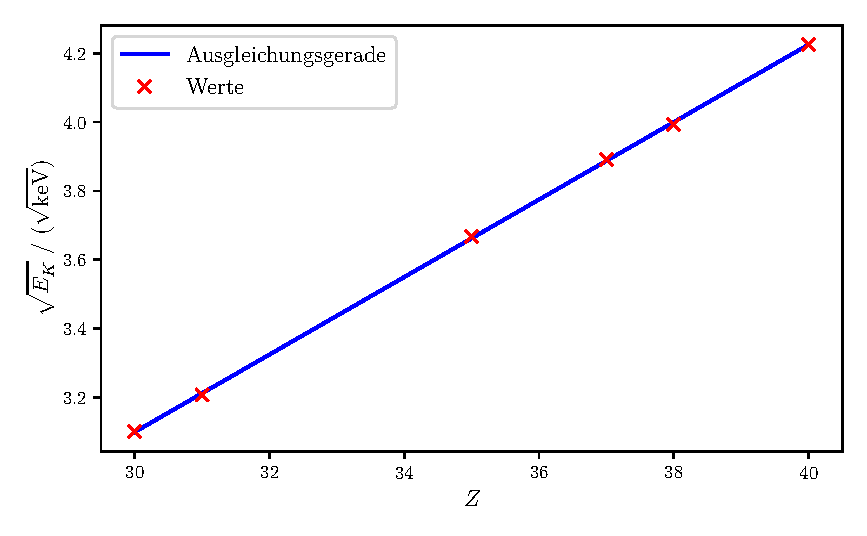
\includegraphics{Rydberg.pdf}
  \caption{Grafik zur Bestimmung der Rydbergkonstanten.}
  \label{fig:Rydberg}
\end{figure}

Die Ausgleichungsgerade hat die Form:
\begin{equation}
 y=a\cdot t+b 
\end{equation}
mit \(y=\sqrt{E_K}\), \(t=Z\), \(a=\sqrt{Rh}\) und \(b=\sigma\sqrt{Rh}\) .\\
Die Parameter ergeben sich zu
\begin{align*}
  a &=(0,112567 \pm 0,000642)\,\mathrm{\sqrt{keV}} \\
  b &=(-0,277592 \pm 0,022702)\,\mathrm{\sqrt{keV}} .\\
 \end{align*}
 Der Fehler für die Rydbergfrequenz $R$  wird dabei über die Gau"s´sche Fehlerfortfplanzung 
 \begin{equation}
     \Delta f = \sqrt{\sum_{i=1}^N {\Bigl(\frac{\partial f}{\partial y_i}\Bigr)^2 (\Delta y_i)^2}}
 \end{equation}

 \begin{align*}
  \Delta R =\sqrt{\Bigl(\frac{1}{h} \cdot 2a \cdot \Delta a\Bigr)^2}
 \end{align*}
 berechnet.
 Somit ergibt der Wert von der Rydbergfrequenz zu
 \begin{align*}
   R =(3,0598 \pm 0,0349) \cdot 10^{15}\,\mathrm{Hz}.
 \end{align*}
 Die Rydbergenergie ist dann \(R_{\infty}=h\cdot R= (12,6714 \pm 0,1445)\,\mathrm{eV}\).
